\newcommand{\spuli}{\text{spüli}}
\newcommand{\wasser}{\text{wasser}}
\subsection{Aufstieg von Luftblasen}
	\subsubsection{Dichte des Spülmittels}
		Nach dem Archimedischen Prinzip ist die Auftriebskraft, die die Flasche ins Wasser hält, gleich die Gewicht des verdrängten Wasser. Somit gilt:
		\begin{equation}
			F_A = \rho_\wasser V_\wasser g
		\end{equation}
		Da die Flasche im Wasser schwimmt, also ist die Flasche im Gleichgewicht und es gilt:
		\begin{align}
			F_G &= F_A \\
			\rho_\spuli V_\spuli \cancel{g} &= \rho_\wasser V_\wasser \cancel{g} \\
			\rho_\spuli &= \rho_\wasser \frac{V_\wasser}{V_\spuli}
		\end{align}
		Dabei ist die Volumen des verdrängtes Wasser als $V_\wasser = \SI{650(50)}{\centi\meter\cubed}$.

		\begin{wrapfigure}{o}{0.4\textwidth}
			\centering
			\vspace{-1em}
			\captionsetup{width=0.4\textwidth, justification=centering}
			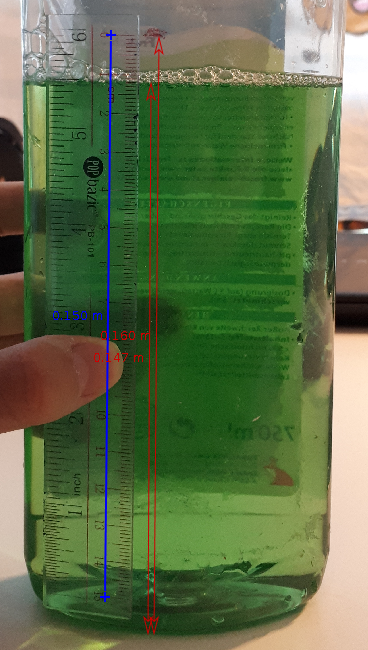
\includegraphics[width=0.25\textwidth]{tv1-dichte-auswertung.png}
			\caption{Messungen der Höhe des Wasserpegels in \tracker{}}
			\vspace{-3em}
		\end{wrapfigure}
		Wir nehmen an, dass der Flasche die Querschnittsfläche für den unteren Teil überall gleich ist, somit ist das Volumen proportional zur Höhe und wir erhalten:
		\begin{align}
			\rho_\spuli &= \rho_\wasser \frac{h_\wasser}{h_\spuli}
		\end{align}
		mit dem entsprechen Fehler:
		\begin{align}
			\Delta \rho_\spuli = \rho_\spuli \relquad{h_\wasser,h_\spuli}
		\end{align}
		Aus \tracker{} und The Engineering Toolbox\footnote{\url{www.engineeringtoolbox.com/water-density-specific-weight-d\_595.html?vA=29&units=C\#}} haben wir als Werten:
		\begin{equation*}
			\begin{tabu}{llr}
				\toprule
				\text{Höhe des Wasserpegels} & h_\wasser & \SI{0.160(5)}{\meter} \\
				\text{Höhe des Spülmittels} & h_\spuli & \SI{0.147(5)}{\meter} \\
				\text{Wasserdichte bei \SI{29}{\celsius}} & \rho_\wasser & \SI{995.96}{\kilo\gram\per\meter\cubed} \\
				\bottomrule
			\end{tabu}
		\end{equation*}
		Damit gilt:
		\begin{align}
			\rho_\spuli &= \SI{995.96}{\kilo\gram\per\meter\cubed} \frac{\SI{0.160}{\meter}}{\SI{0.147}{\meter} }
			= \SI{1084.04}{\kilo\gram\per\meter\cubed} \sigfig{6} \\
			\Delta \rho &= \SI{995.96}{\kilo\gram\per\meter\cubed} \frac{\SI{0.160}{\meter}}{\SI{0.147}{\meter} } 
			\sqrt{\left( \frac{\SI{0.005}{\meter}}{\SI{0.160}{\meter}} \right)^2 + \left( \frac{\SI{0.005}{\meter}}{\SI{0.147}{\meter}} \right)^2} 
			= \SI{50.0714}{\kilo\gram\per\meter\cubed} \sigfig{6}
		\end{align}
		Folglich haben wir eine Dichte von $\rho_\spuli = \SI{1080(60)}{\kilo\gram\per\meter\cubed} = \SI{1.08(6)}{\gram\per\centi\meter\cubed}$.
		\newpage
		Im Vergleich zum Literaturwert\footnote{\url{daten.oehme-lorito.de/sdb/frosch\%20geschirrsp\%C3\%BClmittel\%20limonen.pdf}} haben wir:
		\begin{center}
			\begin{tabular}{lrr}
				\toprule
				Quelle & Temperatur & Wert$/\si{\gram\per\centi\meter\cubed}$ \\
				\midrule
				Experiment & \SI{29(1)}{\celsius}& \num{1.08(6)} \\
				Aräometer   & $\approx$ \SI{23}{\celsius} & \num{1.024(1)} \\
				Hersteller & \SI{20}{\celsius} & \num{1.025} \\
				\bottomrule
			\end{tabular}
		\end{center}
		Die von Aräometer ermittelte Dichte stimmt mit dem Literaturwert überein. Unser experimenteller Wert ist aber nur verträglich mit der anderen zwei Werten. Dieser Unterschied liegt vermutlich daran, dass das Gewicht der Flasche nicht berücksichtigt war. Am Boden der Flasche gibt es auch eine Aussparung, was auch nicht berücksichtigt war. 

	\newpage
	\subsubsection{Viskosität des warmen Spülmittels}
		Die Aufnahmen wurden erst mit \texttt{ffmpeg} geschnittet, bevor sie im \tracker{} geladen sind. Dadurch ist die Anzahl der Frames für jeden Verlauf niedrig gehalten und \tracker{} kann somit schneller die Videos verarbeiten.

		Zur Messung des Durchmessers $2r$ wurden $5$ Messungen mit der "Measuring Tape" Funktion in \tracker{} durchgeführt. Der Mittelwert und die Standardabweichung wurden dann mit LibreOffice Calc berechnet. Dazu sind die Funktionen \texttt{AVERAGE} und \texttt{STDEV} verwendet. Die Standardabweichung entspricht dann die Unsicherheit des Durchmessers:
		\begin{center}
			\begin{tabular}{l*{6}{r}}
				\toprule
				Blase & $2r_1/\si{\milli\meter}$ & $2r_2/\si{\milli\meter}$ & $2r_3/\si{\milli\meter}$ & $2r_4/\si{\milli\meter}$ & $2r_5/\si{\milli\meter}$ & $\overline{(2r)}/\si{\milli\meter}$ \\
				\midrule
				\num{1} & \num{2.753} & \num{2.810} & \num{2.890} & \num{2.814} & \num{2.920}  & \num{2.84(7)} \\
				\num{2} & \num{2.664} & \num{2.629} & \num{2.632} & \num{2.593} & \num{2.645}  & \num{2.633(27)} \\
				\num{3} & \num{3.033} & \num{3.073} & \num{3.014} & \num{2.973} & \num{3.117}  & \num{3.04(6)} \\
				\num{4} & \num{2.675} & \num{2.769} & \num{2.725} & \num{2.501} & \num{2.545}  & \num{2.64(12)} \\
				\num{5} & \num{3.423} & \num{3.463} & \num{3.539} & \num{3.547} & \num{3.502}  & \num{3.49(6)} \\
				\num{6} & \num{3.537} & \num{3.586} & \num{3.597} & \num{3.501} & \num{3.595}  & \num{3.56(5)} \\
				\num{7} & \num{7.351} & \num{6.899} & \num{6.953} & \num{7.407} & \num{6.916}  & \num{7.11(26)} \\
				\num{8} & \num{5.511} & \num{5.774} & \num{5.368} & \num{5.721} & \num{5.472}  & \num{5.57(18)} \\
				\num{9} & \num{2.939} & \num{2.640} & \num{2.693} & \num{2.724} & \num{2.770}  & \num{2.75(12)} \\
				\num{10} & \num{3.641} & \num{3.797} & \num{3.858} & \num{3.733} & \num{3.668} & \num{3.74(9)} \\
				\bottomrule
			\end{tabular}
		\end{center}

		Die erhaltene Zeit-Position Daten aus \tracker{} sind mit \gnuplot{} geplottet und es wurde eine Kurveanpassung zur $y = mt + c~$ für jede Blase durchgeführt. Da \tracker{} keine explizite Unsicherheit ermittelt, vernachlässigen wir sie für die Kurvenanpassung.

		Für das genaue \gnuplot{} Code, siehe Appendix \ref{appdx:tvone}. 
		% https://tex.stackexchange.com/a/98142
		\begin{figure}[H]
			\centering
			\captionsetup{width=0.8\textwidth, justification=centering}
			\resizebox{\linewidth}{!}{% GNUPLOT: LaTeX picture with Postscript
\begingroup
  \makeatletter
  \providecommand\color[2][]{%
    \GenericError{(gnuplot) \space\space\space\@spaces}{%
      Package color not loaded in conjunction with
      terminal option `colourtext'%
    }{See the gnuplot documentation for explanation.%
    }{Either use 'blacktext' in gnuplot or load the package
      color.sty in LaTeX.}%
    \renewcommand\color[2][]{}%
  }%
  \providecommand\includegraphics[2][]{%
    \GenericError{(gnuplot) \space\space\space\@spaces}{%
      Package graphicx or graphics not loaded%
    }{See the gnuplot documentation for explanation.%
    }{The gnuplot epslatex terminal needs graphicx.sty or graphics.sty.}%
    \renewcommand\includegraphics[2][]{}%
  }%
  \providecommand\rotatebox[2]{#2}%
  \@ifundefined{ifGPcolor}{%
    \newif\ifGPcolor
    \GPcolortrue
  }{}%
  \@ifundefined{ifGPblacktext}{%
    \newif\ifGPblacktext
    \GPblacktexttrue
  }{}%
  % define a \g@addto@macro without @ in the name:
  \let\gplgaddtomacro\g@addto@macro
  % define empty templates for all commands taking text:
  \gdef\gplbacktext{}%
  \gdef\gplfronttext{}%
  \makeatother
  \ifGPblacktext
    % no textcolor at all
    \def\colorrgb#1{}%
    \def\colorgray#1{}%
  \else
    % gray or color?
    \ifGPcolor
      \def\colorrgb#1{\color[rgb]{#1}}%
      \def\colorgray#1{\color[gray]{#1}}%
      \expandafter\def\csname LTw\endcsname{\color{white}}%
      \expandafter\def\csname LTb\endcsname{\color{black}}%
      \expandafter\def\csname LTa\endcsname{\color{black}}%
      \expandafter\def\csname LT0\endcsname{\color[rgb]{1,0,0}}%
      \expandafter\def\csname LT1\endcsname{\color[rgb]{0,1,0}}%
      \expandafter\def\csname LT2\endcsname{\color[rgb]{0,0,1}}%
      \expandafter\def\csname LT3\endcsname{\color[rgb]{1,0,1}}%
      \expandafter\def\csname LT4\endcsname{\color[rgb]{0,1,1}}%
      \expandafter\def\csname LT5\endcsname{\color[rgb]{1,1,0}}%
      \expandafter\def\csname LT6\endcsname{\color[rgb]{0,0,0}}%
      \expandafter\def\csname LT7\endcsname{\color[rgb]{1,0.3,0}}%
      \expandafter\def\csname LT8\endcsname{\color[rgb]{0.5,0.5,0.5}}%
    \else
      % gray
      \def\colorrgb#1{\color{black}}%
      \def\colorgray#1{\color[gray]{#1}}%
      \expandafter\def\csname LTw\endcsname{\color{white}}%
      \expandafter\def\csname LTb\endcsname{\color{black}}%
      \expandafter\def\csname LTa\endcsname{\color{black}}%
      \expandafter\def\csname LT0\endcsname{\color{black}}%
      \expandafter\def\csname LT1\endcsname{\color{black}}%
      \expandafter\def\csname LT2\endcsname{\color{black}}%
      \expandafter\def\csname LT3\endcsname{\color{black}}%
      \expandafter\def\csname LT4\endcsname{\color{black}}%
      \expandafter\def\csname LT5\endcsname{\color{black}}%
      \expandafter\def\csname LT6\endcsname{\color{black}}%
      \expandafter\def\csname LT7\endcsname{\color{black}}%
      \expandafter\def\csname LT8\endcsname{\color{black}}%
    \fi
  \fi
    \setlength{\unitlength}{0.0500bp}%
    \ifx\gptboxheight\undefined%
      \newlength{\gptboxheight}%
      \newlength{\gptboxwidth}%
      \newsavebox{\gptboxtext}%
    \fi%
    \setlength{\fboxrule}{0.5pt}%
    \setlength{\fboxsep}{1pt}%
\begin{picture}(17280.00,11520.00)%
    \gplgaddtomacro\gplbacktext{%
      \csname LTb\endcsname%%
      \put(946,704){\makebox(0,0)[r]{\strut{}$-100$}}%
      \put(946,1627){\makebox(0,0)[r]{\strut{}$0$}}%
      \put(946,2550){\makebox(0,0)[r]{\strut{}$100$}}%
      \put(946,3474){\makebox(0,0)[r]{\strut{}$200$}}%
      \put(946,4397){\makebox(0,0)[r]{\strut{}$300$}}%
      \put(946,5320){\makebox(0,0)[r]{\strut{}$400$}}%
      \put(946,6243){\makebox(0,0)[r]{\strut{}$500$}}%
      \put(946,7166){\makebox(0,0)[r]{\strut{}$600$}}%
      \put(946,8089){\makebox(0,0)[r]{\strut{}$700$}}%
      \put(946,9013){\makebox(0,0)[r]{\strut{}$800$}}%
      \put(946,9936){\makebox(0,0)[r]{\strut{}$900$}}%
      \put(946,10859){\makebox(0,0)[r]{\strut{}$1000$}}%
      \put(1078,484){\makebox(0,0){\strut{}$0$}}%
      \put(2659,484){\makebox(0,0){\strut{}$1$}}%
      \put(4239,484){\makebox(0,0){\strut{}$2$}}%
      \put(5820,484){\makebox(0,0){\strut{}$3$}}%
      \put(7400,484){\makebox(0,0){\strut{}$4$}}%
      \put(8981,484){\makebox(0,0){\strut{}$5$}}%
      \put(10561,484){\makebox(0,0){\strut{}$6$}}%
      \put(12142,484){\makebox(0,0){\strut{}$7$}}%
      \put(13722,484){\makebox(0,0){\strut{}$8$}}%
      \put(15303,484){\makebox(0,0){\strut{}$9$}}%
      \put(16883,484){\makebox(0,0){\strut{}$10$}}%
    }%
    \gplgaddtomacro\gplfronttext{%
      \csname LTb\endcsname%%
      \put(209,5781){\rotatebox{-270}{\makebox(0,0){\strut{}Vertikale Position $y/\si{\milli\meter}$}}}%
      \put(8980,154){\makebox(0,0){\strut{}Zeit $t/\si{\second}$}}%
      \csname LTb\endcsname%%
      \put(1210,10653){\makebox(0,0)[l]{\strut{}Blase 1}}%
      \csname LTb\endcsname%%
      \put(1210,10367){\makebox(0,0)[l]{\strut{}Blase 2}}%
      \csname LTb\endcsname%%
      \put(1210,10081){\makebox(0,0)[l]{\strut{}Blase 3}}%
      \csname LTb\endcsname%%
      \put(1210,9795){\makebox(0,0)[l]{\strut{}Blase 4}}%
      \csname LTb\endcsname%%
      \put(1210,9509){\makebox(0,0)[l]{\strut{}Blase 5}}%
      \csname LTb\endcsname%%
      \put(1210,9223){\makebox(0,0)[l]{\strut{}Blase 6}}%
      \csname LTb\endcsname%%
      \put(1210,8937){\makebox(0,0)[l]{\strut{}Blase 7}}%
      \csname LTb\endcsname%%
      \put(1210,8651){\makebox(0,0)[l]{\strut{}Blase 8}}%
      \csname LTb\endcsname%%
      \put(1210,8365){\makebox(0,0)[l]{\strut{}Blase 9}}%
      \csname LTb\endcsname%%
      \put(1210,8079){\makebox(0,0)[l]{\strut{}Blase 10}}%
      \csname LTb\endcsname%%
      \put(1210,7793){\makebox(0,0)[l]{\strut{}$18,75936t + (0,83453)$}}%
      \csname LTb\endcsname%%
      \put(1210,7507){\makebox(0,0)[l]{\strut{}$14,88056t + (0,39407)$}}%
      \csname LTb\endcsname%%
      \put(1210,7221){\makebox(0,0)[l]{\strut{}$23,80945t + (0,10412)$}}%
      \csname LTb\endcsname%%
      \put(1210,6935){\makebox(0,0)[l]{\strut{}$14,78785t + (-1,55167)$}}%
      \csname LTb\endcsname%%
      \put(1210,6649){\makebox(0,0)[l]{\strut{}$28,05332t + (-2,10395)$}}%
      \csname LTb\endcsname%%
      \put(1210,6363){\makebox(0,0)[l]{\strut{}$35,18369t + (1,75442)$}}%
      \csname LTb\endcsname%%
      \put(1210,6077){\makebox(0,0)[l]{\strut{}$99,39234t + (0,47523)$}}%
      \csname LTb\endcsname%%
      \put(1210,5791){\makebox(0,0)[l]{\strut{}$67,19169t + (1,10226)$}}%
      \csname LTb\endcsname%%
      \put(1210,5505){\makebox(0,0)[l]{\strut{}$17,52108t + (-0,18687)$}}%
      \csname LTb\endcsname%%
      \put(1210,5219){\makebox(0,0)[l]{\strut{}$36,19531t + (0,01841)$}}%
      \csname LTb\endcsname%%
      \put(8980,11189){\makebox(0,0){\strut{}Aufstiegsverlauf der Blasen (Warm)}}%
    }%
    \gplbacktext
    \put(0,0){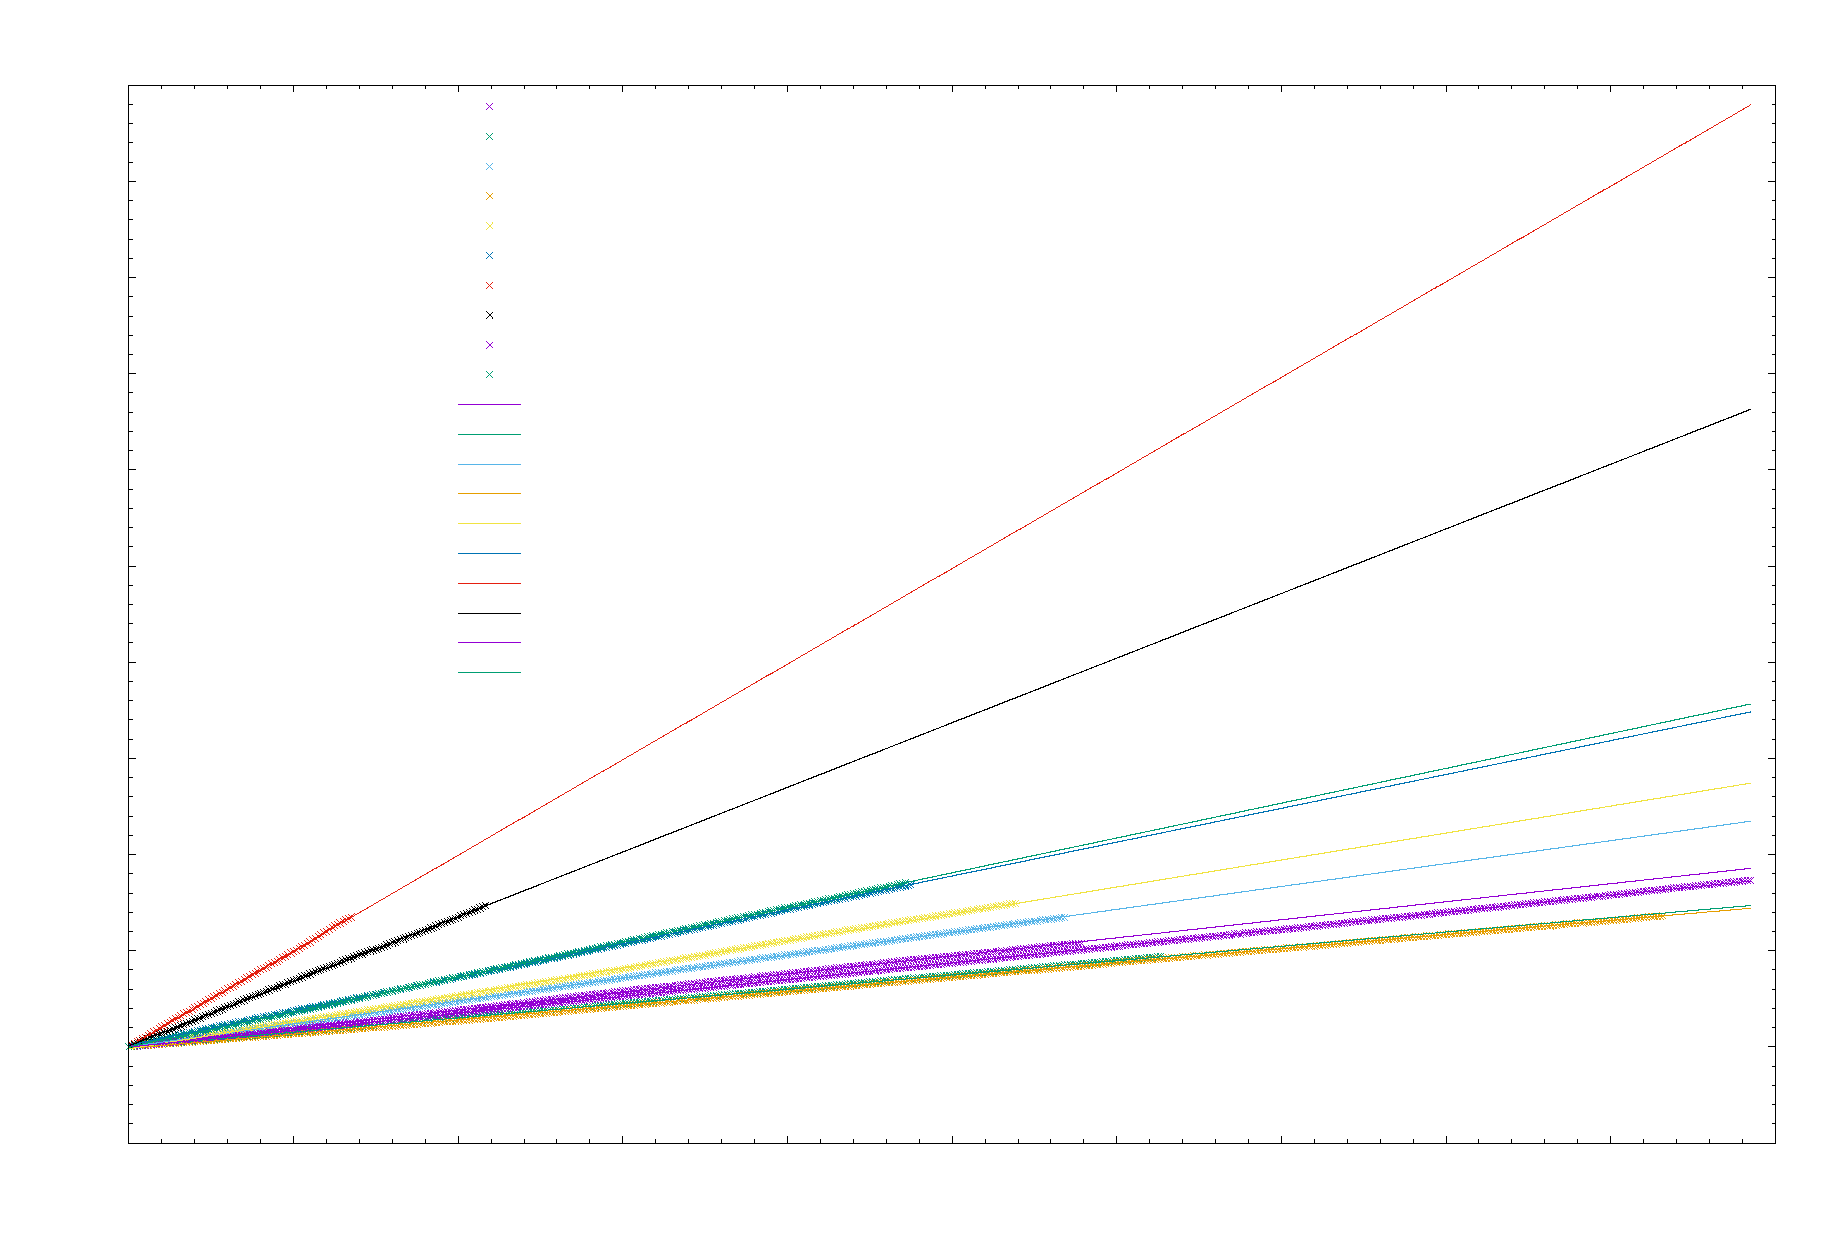
\includegraphics[width={864.00bp},height={576.00bp}]{tv1-plot-warm}}%
    \gplfronttext
  \end{picture}%
\endgroup
}
			\caption{Aufstieg der Luftblasen \textattachfile[author={Yudong Sun},color={0 0.404 0.584},description={.zip Datei mit der Messwerten},mimetype={application/zip},timezone={+02'00'}]{./attachments/luftblasen-warm.zip}{\textit{(Daten)}}}
			\vspace{-1em}
		\end{figure}
		Als Endergebnis erhalten wir:
		\begin{center}
			\begin{tabular}{lrrr}
				\toprule
				Blase Nr. & $m/\si{\milli\meter\per\second}$ & $c/\si{\milli\meter}$ & $\chi^2_\text{red}$ \\
				\midrule
					$1$ &  \num{18,75936(1679)} & \num{0,83453(5611)} & \num{0,27505} \\
					$2$ &  \num{14,88056(310)} & \num{0,39407(1123)} & \num{0,01194} \\
					$3$ &  \num{23,80945(1052)} & \num{0,10412(3453)} & \num{0,10242} \\
					$4$ &  \num{14,78785(770)} & \num{-1,55167(4144)} & \num{0,24111} \\
					$5$ &  \num{28,05332(3272)} & \num{-2,10395(10176)} & \num{0,84266} \\
					$6$ &  \num{35,18369(1851)} & \num{1,75442(5080)} & \num{0,18549} \\
					$7$ &  \num{99,39234(14013)} & \num{0,47523(10955)} & \num{0,25057} \\
					$8$ &  \num{67,19169(8685)} & \num{1,10226(10885)} & \num{0,39251} \\
					$9$ &  \num{17,52108(486)} & \num{-0,18687(2767)} & \num{0,11364} \\
					$10$ & \num{36,19531(880)} & \num{0,01841(2399)} & \num{0,04108} \\
				\bottomrule
			\end{tabular}
		\end{center}
		Aus der niedrigen $\chi^2_\text{red}$ sind alle Kurveanpassungen gut. $m$ entspricht in diesem Fall die Geschwindigkeit $v$.
		Laut der Anleitung gilt:
		\begin{align}
			\eta_\spuli &= \frac{2\cdot g\rho_\spuli}{9\cdot v_\text{Luftblase}}\cdot r^2_\text{Luftblase} = \frac{g\cdot \rho_\spuli}{18\cdot v_\text{Luftblase}}\cdot (2r_\text{Luftblase})^2 \label{eqn:warm-eta} \\
			\Delta \eta_\spuli &= \eta_\spuli \sqrt{
				\left(\frac{\Delta \rho_\spuli}{\rho_\spuli}\right)^2 +
				\left(\frac{\Delta v_\text{Luftblase}}{v_\text{Luftblase}}\right)^2 +
				\left(2\frac{\Delta (2r_\text{Luftblase})}{2r_\text{Luftblase}}\right)^2
			} \label{eqn:warm-delta-eta}
		\end{align}
		Die Viskositäten und die entsprechenden Fehler wurden dann mittels LibreOffice Calc anhand \eqref{eqn:warm-eta} und \eqref{eqn:warm-delta-eta} berechnet. Die genaue Rechnung sind wegen Übersichtlichkeit hier ausgelassen.

		Als Ergebnis erhalten wir:
		\begin{center}
			\begin{tabular}{lrrr}
				\toprule
				Blase Nr. $i$ & $2r_i/\si{\milli\meter}$ & $v_i/\si{\milli\meter\per\second}$ & $\eta_i/\si{\milli\pascal\second}$ \\
				\midrule
				\num{1} & \num{2.84(7)} & \num{18.759(17)} & \num{253(19)} \\
				\num{2} & \num{2.633(27)} & \num{14.881(4)} & \num{274(17)} \\
				\num{3} & \num{3.04(6)} & \num{23.809(11)} & \num{228(16)} \\
				\num{4} & \num{2.64(12)} & \num{14.788(8)} & \num{280(30)} \\
				\num{5} & \num{3.49(6)} & \num{28.05(4)} & \num{256(17)} \\
				\num{6} & \num{3.56(5)} & \num{35.18(2)} & \num{212(14)} \\
				\num{7} & \num{7.11(26)} & \num{99.39(15)} & \num{299(28)} \\
				\num{8} & \num{5.57(18)} & \num{67.19(9)} & \num{272(24)} \\
				\num{9} & \num{2.75(12)} & \num{17.521(5)} & \num{254(27)} \\
				\num{10} & \num{3.74(9)} & \num{36.195(9)} & \num{227(17)} \\
				\bottomrule
			\end{tabular}
		\end{center}
		Der Mittelwert $\overline{\eta}$ ist dann gegeben durch:
		\begin{align}
			\overline{\eta} = \frac{1}{10}\sum^{10}_{i=1}\eta_i  && \text{mit} && \Delta \overline{\eta} = \frac{1}{10} \sqrt{\sum^{10}_{i=1}(\Delta\eta_i)^2} \label{eqn:avg-eta-warm}
		\end{align}
		und die Standardabweichung:
		\begin{align}
			s(\eta) = \sqrt{\frac{1}{10 - 1} \sum^{10}_{i=1}(\eta_i - \overline{\eta})^2}
			\label{eqn:stdev-eta-warm}
		\end{align}
		Die genaue Rechnungen erfolgen anhand \eqref{eqn:avg-eta-warm} und \eqref{eqn:stdev-eta-warm} in LibreOffice Calc und sind wegen Über\-sicht\-lich\-keit hier ausgelassen. Für den Mittelwert und die Standabweichung sind die Funktionen \texttt{AVERAGE} und \texttt{STDEV.S} direkt verwendet. Wir erhalten:
		\begin{center}
			\begin{tabular}{lrr}
				\toprule
				Mittelwert & $\overline{\eta}$ & \SI{255.5}{\milli\pascal\second}\\
				Unsicherheit des Mittelwertes & $\Delta\overline{\eta}$ & \SI{6.9}{\milli\pascal\second}\\
				Standardabweichung & $s(\eta)$ & \SI{28}{\milli\pascal\second}\\
				\bottomrule
			\end{tabular}
		\end{center}
		wobei $\Delta\overline{\eta}$ und $s(\eta)$ beides aufgerundet sind. 

		Da die Standardabweichung größer als die Unsicherheit des Mittelwertes ist, nehmen wir die Standardabweichung als Fehler und erhalten für $T = \SI{29(1)}{\celsius}$ eine Viskosität von $\eta = \SI{256(28)}{\milli\pascal\second}$.

	\subsubsection{Viskosität des kalten Spülmittels}
		Wir wiederholen nun alle Rechnungen für das kalte Spülmittel. Sodass die Variablen nicht durcheinander kommen, sind die Auswertung zum kalten Spülmittel hier im zweiten Abschnitt geteilt. 

		Es ist davon ausgegangen, dass die Dichte des Spülmittels nicht Temperaturabhängig ist.

		
		
	\subsubsection{Diskussion}
		biggest error = dichte